\documentclass[1p]{elsarticle_modified}
%\bibliographystyle{elsarticle-num}

%\usepackage[colorlinks]{hyperref}
%\usepackage{abbrmath_seonhwa} %\Abb, \Ascr, \Acal ,\Abf, \Afrak
\usepackage{amsfonts}
\usepackage{amssymb}
\usepackage{amsmath}
\usepackage{amsthm}
\usepackage{scalefnt}
\usepackage{amsbsy}
\usepackage{kotex}
\usepackage{caption}
\usepackage{subfig}
\usepackage{color}
\usepackage{graphicx}
\usepackage{xcolor} %% white, black, red, green, blue, cyan, magenta, yellow
\usepackage{float}
\usepackage{setspace}
\usepackage{hyperref}

\usepackage{tikz}
\usetikzlibrary{arrows}

\usepackage{multirow}
\usepackage{array} % fixed length table
\usepackage{hhline}

%%%%%%%%%%%%%%%%%%%%%
\makeatletter
\renewcommand*\env@matrix[1][\arraystretch]{%
	\edef\arraystretch{#1}%
	\hskip -\arraycolsep
	\let\@ifnextchar\new@ifnextchar
	\array{*\c@MaxMatrixCols c}}
\makeatother %https://tex.stackexchange.com/questions/14071/how-can-i-increase-the-line-spacing-in-a-matrix
%%%%%%%%%%%%%%%

\usepackage[normalem]{ulem}

\newcommand{\msout}[1]{\ifmmode\text{\sout{\ensuremath{#1}}}\else\sout{#1}\fi}
%SOURCE: \msout is \stkout macro in https://tex.stackexchange.com/questions/20609/strikeout-in-math-mode

\newcommand{\cancel}[1]{
	\ifmmode
	{\color{red}\msout{#1}}
	\else
	{\color{red}\sout{#1}}
	\fi
}

\newcommand{\add}[1]{
	{\color{blue}\uwave{#1}}
}

\newcommand{\replace}[2]{
	\ifmmode
	{\color{red}\msout{#1}}{\color{blue}\uwave{#2}}
	\else
	{\color{red}\sout{#1}}{\color{blue}\uwave{#2}}
	\fi
}

\newcommand{\Sol}{\mathcal{S}} %segment
\newcommand{\D}{D} %diagram
\newcommand{\A}{\mathcal{A}} %arc


%%%%%%%%%%%%%%%%%%%%%%%%%%%%%5 test

\def\sl{\operatorname{\textup{SL}}(2,\Cbb)}
\def\psl{\operatorname{\textup{PSL}}(2,\Cbb)}
\def\quan{\mkern 1mu \triangleright \mkern 1mu}

\theoremstyle{definition}
\newtheorem{thm}{Theorem}[section]
\newtheorem{prop}[thm]{Proposition}
\newtheorem{lem}[thm]{Lemma}
\newtheorem{ques}[thm]{Question}
\newtheorem{cor}[thm]{Corollary}
\newtheorem{defn}[thm]{Definition}
\newtheorem{exam}[thm]{Example}
\newtheorem{rmk}[thm]{Remark}
\newtheorem{alg}[thm]{Algorithm}

\newcommand{\I}{\sqrt{-1}}
\begin{document}

%\begin{frontmatter}
%
%\title{Boundary parabolic representations of knots up to 8 crossings}
%
%%% Group authors per affiliation:
%\author{Yunhi Cho} 
%\address{Department of Mathematics, University of Seoul, Seoul, Korea}
%\ead{yhcho@uos.ac.kr}
%
%
%\author{Seonhwa Kim} %\fnref{s_kim}}
%\address{Center for Geometry and Physics, Institute for Basic Science, Pohang, 37673, Korea}
%\ead{ryeona17@ibs.re.kr}
%
%\author{Hyuk Kim}
%\address{Department of Mathematical Sciences, Seoul National University, Seoul 08826, Korea}
%\ead{hyukkim@snu.ac.kr}
%
%\author{Seokbeom Yoon}
%\address{Department of Mathematical Sciences, Seoul National University, Seoul, 08826,  Korea}
%\ead{sbyoon15@snu.ac.kr}
%
%\begin{abstract}
%We find all boundary parabolic representation of knots up to 8 crossings.
%
%\end{abstract}
%\begin{keyword}
%    \MSC[2010] 57M25 
%\end{keyword}
%
%\end{frontmatter}

%\linenumbers
%\tableofcontents
%
\newcommand\colored[1]{\textcolor{white}{\rule[-0.35ex]{0.8em}{1.4ex}}\kern-0.8em\color{red} #1}%
%\newcommand\colored[1]{\textcolor{white}{ #1}\kern-2.17ex	\textcolor{white}{ #1}\kern-1.81ex	\textcolor{white}{ #1}\kern-2.15ex\color{red}#1	}

{\Large $\underline{12n_{0683}~(K12n_{0683})}$}

\setlength{\tabcolsep}{10pt}
\renewcommand{\arraystretch}{1.6}
\vspace{1cm}\begin{tabular}{m{100pt}>{\centering\arraybackslash}m{274pt}}
\multirow{5}{120pt}{
	\centering
	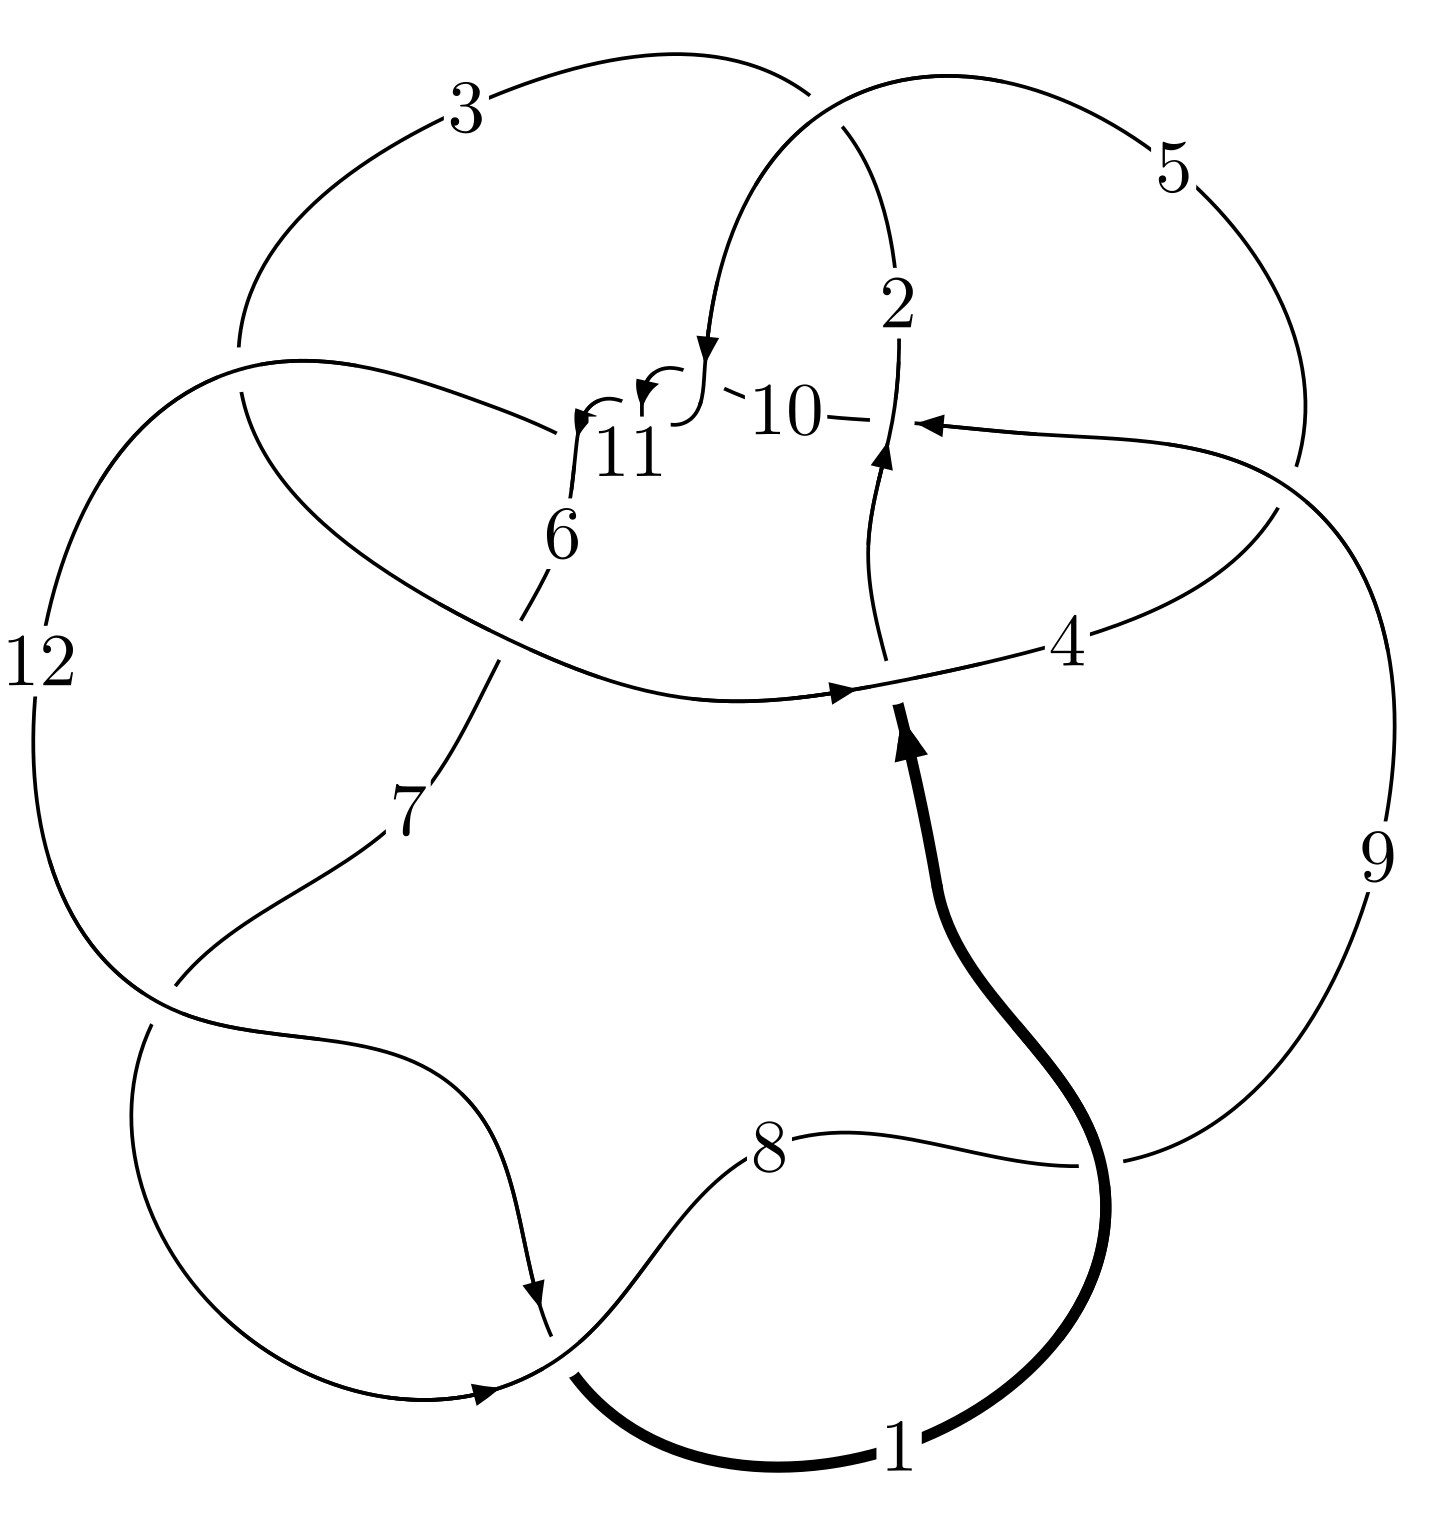
\includegraphics[width=112pt]{../../../GIT/diagram.site/Diagrams/png/2772_12n_0683.png}\\
\ \ \ A knot diagram\footnotemark}&
\allowdisplaybreaks
\textbf{Linearized knot diagam} \\
\cline{2-2}
 &
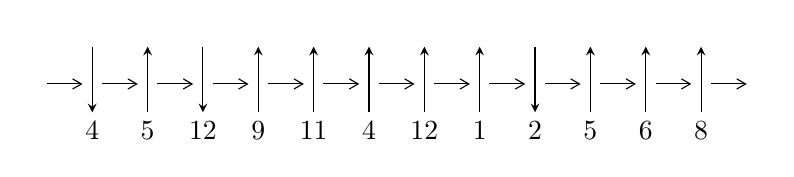
\begin{tikzpicture}[x=20pt, y=17pt]
	% nodes
	\node (C0) at (0, 0) {};
	\node (C1) at (1, 0) {};
	\node (C1U) at (1, +1) {};
	\node (C1D) at (1, -1) {4};

	\node (C2) at (2, 0) {};
	\node (C2U) at (2, +1) {};
	\node (C2D) at (2, -1) {5};

	\node (C3) at (3, 0) {};
	\node (C3U) at (3, +1) {};
	\node (C3D) at (3, -1) {12};

	\node (C4) at (4, 0) {};
	\node (C4U) at (4, +1) {};
	\node (C4D) at (4, -1) {9};

	\node (C5) at (5, 0) {};
	\node (C5U) at (5, +1) {};
	\node (C5D) at (5, -1) {11};

	\node (C6) at (6, 0) {};
	\node (C6U) at (6, +1) {};
	\node (C6D) at (6, -1) {4};

	\node (C7) at (7, 0) {};
	\node (C7U) at (7, +1) {};
	\node (C7D) at (7, -1) {12};

	\node (C8) at (8, 0) {};
	\node (C8U) at (8, +1) {};
	\node (C8D) at (8, -1) {1};

	\node (C9) at (9, 0) {};
	\node (C9U) at (9, +1) {};
	\node (C9D) at (9, -1) {2};

	\node (C10) at (10, 0) {};
	\node (C10U) at (10, +1) {};
	\node (C10D) at (10, -1) {5};

	\node (C11) at (11, 0) {};
	\node (C11U) at (11, +1) {};
	\node (C11D) at (11, -1) {6};

	\node (C12) at (12, 0) {};
	\node (C12U) at (12, +1) {};
	\node (C12D) at (12, -1) {8};
	\node (C13) at (13, 0) {};

	% arrows
	\draw[->,>={angle 60}]
	(C0) edge (C1) (C1) edge (C2) (C2) edge (C3) (C3) edge (C4) (C4) edge (C5) (C5) edge (C6) (C6) edge (C7) (C7) edge (C8) (C8) edge (C9) (C9) edge (C10) (C10) edge (C11) (C11) edge (C12) (C12) edge (C13) ;	\draw[->,>=stealth]
	(C1U) edge (C1D) (C2D) edge (C2U) (C3U) edge (C3D) (C4D) edge (C4U) (C5D) edge (C5U) (C6D) edge (C6U) (C7D) edge (C7U) (C8D) edge (C8U) (C9U) edge (C9D) (C10D) edge (C10U) (C11D) edge (C11U) (C12D) edge (C12U) ;
	\end{tikzpicture} \\
\hhline{~~} \\& 
\textbf{Solving Sequence} \\ \cline{2-2} 
 &
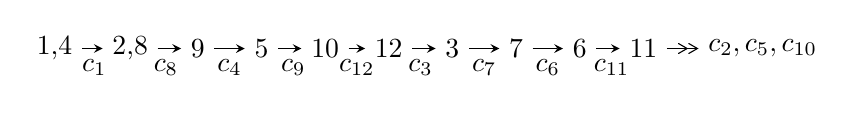
\begin{tikzpicture}[x=23pt, y=7pt]
	% node
	\node (A0) at (-1/8, 0) {1,4};
	\node (A1) at (17/16, 0) {2,8};
	\node (A2) at (17/8, 0) {9};
	\node (A3) at (25/8, 0) {5};
	\node (A4) at (33/8, 0) {10};
	\node (A5) at (41/8, 0) {12};
	\node (A6) at (49/8, 0) {3};
	\node (A7) at (57/8, 0) {7};
	\node (A8) at (65/8, 0) {6};
	\node (A9) at (73/8, 0) {11};
	\node (C1) at (1/2, -1) {$c_{1}$};
	\node (C2) at (13/8, -1) {$c_{8}$};
	\node (C3) at (21/8, -1) {$c_{4}$};
	\node (C4) at (29/8, -1) {$c_{9}$};
	\node (C5) at (37/8, -1) {$c_{12}$};
	\node (C6) at (45/8, -1) {$c_{3}$};
	\node (C7) at (53/8, -1) {$c_{7}$};
	\node (C8) at (61/8, -1) {$c_{6}$};
	\node (C9) at (69/8, -1) {$c_{11}$};
	\node (A10) at (11, 0) {$c_{2},c_{5},c_{10}$};

	% edge
	\draw[->,>=stealth]	
	(A0) edge (A1) (A1) edge (A2) (A2) edge (A3) (A3) edge (A4) (A4) edge (A5) (A5) edge (A6) (A6) edge (A7) (A7) edge (A8) (A8) edge (A9) ;
	\draw[->>,>={angle 60}]	
	(A9) edge (A10);
\end{tikzpicture} \\ 

\end{tabular} \\

\footnotetext{
The image of knot diagram is generated by the software ``\textbf{Draw programme}" developed by Andrew Bartholomew(\url{http://www.layer8.co.uk/maths/draw/index.htm\#Running-draw}), where we modified some parts for our purpose(\url{https://github.com/CATsTAILs/LinksPainter}).
}\phantom \\ \newline 
\centering \textbf{Ideals for irreducible components\footnotemark of $X_{\text{par}}$} 
 
\begin{align*}
I^u_{1}&=\langle 
-2.19867\times10^{203} u^{56}+5.65768\times10^{203} u^{55}+\cdots+1.13098\times10^{204} b-3.04242\times10^{203},\\
\phantom{I^u_{1}}&\phantom{= \langle  }1.01630\times10^{202} u^{56}-2.54589\times10^{202} u^{55}+\cdots+4.34992\times10^{202} a-1.92664\times10^{204},\;u^{57}-2 u^{56}+\cdots+99 u+1\rangle \\
I^u_{2}&=\langle 
-190 u^{12}+1765 u^{11}+\cdots+334 b+209,\;-1291 u^{12}+11918 u^{11}+\cdots+167 a-2972,\\
\phantom{I^u_{2}}&\phantom{= \langle  }u^{13}-9 u^{12}+40 u^{11}-112 u^{10}+212 u^9-270 u^8+213 u^7-70 u^6-43 u^5+56 u^4-13 u^3-10 u^2+3 u+1\rangle \\
\\
\end{align*}
\raggedright * 2 irreducible components of $\dim_{\mathbb{C}}=0$, with total 70 representations.\\
\footnotetext{All coefficients of polynomials are rational numbers. But the coefficients are sometimes approximated in decimal forms when there is not enough margin.}
\newpage
\renewcommand{\arraystretch}{1}
\centering \section*{I. $I^u_{1}= \langle -2.20\times10^{203} u^{56}+5.66\times10^{203} u^{55}+\cdots+1.13\times10^{204} b-3.04\times10^{203},\;1.02\times10^{202} u^{56}-2.55\times10^{202} u^{55}+\cdots+4.35\times10^{202} a-1.93\times10^{204},\;u^{57}-2 u^{56}+\cdots+99 u+1 \rangle$}
\flushleft \textbf{(i) Arc colorings}\\
\begin{tabular}{m{7pt} m{180pt} m{7pt} m{180pt} }
\flushright $a_{1}=$&$\begin{pmatrix}1\\0\end{pmatrix}$ \\
\flushright $a_{4}=$&$\begin{pmatrix}0\\u\end{pmatrix}$ \\
\flushright $a_{2}=$&$\begin{pmatrix}1\\u^2\end{pmatrix}$ \\
\flushright $a_{8}=$&$\begin{pmatrix}-0.233636 u^{56}+0.585272 u^{55}+\cdots+376.156 u+44.2914\\0.194404 u^{56}-0.500246 u^{55}+\cdots-3.13746 u+0.269007\end{pmatrix}$ \\
\flushright $a_{9}=$&$\begin{pmatrix}-0.0392325 u^{56}+0.0850261 u^{55}+\cdots+373.019 u+44.5604\\0.194404 u^{56}-0.500246 u^{55}+\cdots-3.13746 u+0.269007\end{pmatrix}$ \\
\flushright $a_{5}=$&$\begin{pmatrix}-0.709204 u^{56}+1.81312 u^{55}+\cdots+1.23457 u-20.2316\\0.113804 u^{56}-0.292360 u^{55}+\cdots+60.6616 u+0.512414\end{pmatrix}$ \\
\flushright $a_{10}=$&$\begin{pmatrix}-0.206310 u^{56}+0.511643 u^{55}+\cdots+375.546 u+44.2848\\0.152217 u^{56}-0.398947 u^{55}+\cdots-12.1241 u+0.176546\end{pmatrix}$ \\
\flushright $a_{12}=$&$\begin{pmatrix}-0.211474 u^{56}+0.400072 u^{55}+\cdots-355.701 u+11.0408\\-0.300940 u^{56}+0.738560 u^{55}+\cdots-111.054 u-1.10820\end{pmatrix}$ \\
\flushright $a_{3}=$&$\begin{pmatrix}1.16949 u^{56}-2.32458 u^{55}+\cdots+1535.29 u+14.9071\\-0.275037 u^{56}+0.741382 u^{55}+\cdots+63.4359 u+0.800985\end{pmatrix}$ \\
\flushright $a_{7}=$&$\begin{pmatrix}1.71051 u^{56}-3.73781 u^{55}+\cdots+1743.01 u+54.3756\\-0.170202 u^{56}+0.417387 u^{55}+\cdots+3.50097 u+0.427858\end{pmatrix}$ \\
\flushright $a_{6}=$&$\begin{pmatrix}1.71051 u^{56}-3.73781 u^{55}+\cdots+1743.01 u+54.3756\\-0.0441047 u^{56}+0.107941 u^{55}+\cdots+33.1523 u+0.744645\end{pmatrix}$ \\
\flushright $a_{11}=$&$\begin{pmatrix}-0.0330544 u^{56}-0.0970298 u^{55}+\cdots-433.886 u+25.2387\\-0.0307323 u^{56}+0.0397139 u^{55}+\cdots-103.215 u-0.950993\end{pmatrix}$\\&\end{tabular}
\flushleft \textbf{(ii) Obstruction class $= -1$}\\~\\
\flushleft \textbf{(iii) Cusp Shapes $= 1.49472 u^{56}-3.47198 u^{55}+\cdots+455.723 u+19.2896$}\\~\\
\newpage\renewcommand{\arraystretch}{1}
\flushleft \textbf{(iv) u-Polynomials at the component}\newline \\
\begin{tabular}{m{50pt}|m{274pt}}
Crossings & \hspace{64pt}u-Polynomials at each crossing \\
\hline $$\begin{aligned}c_{1}\end{aligned}$$&$\begin{aligned}
&u^{57}+2 u^{56}+\cdots+99 u-1
\end{aligned}$\\
\hline $$\begin{aligned}c_{2}\end{aligned}$$&$\begin{aligned}
&u^{57}+u^{56}+\cdots-217 u+31
\end{aligned}$\\
\hline $$\begin{aligned}c_{3}\end{aligned}$$&$\begin{aligned}
&u^{57}+2 u^{56}+\cdots-3 u-1
\end{aligned}$\\
\hline $$\begin{aligned}c_{4}\end{aligned}$$&$\begin{aligned}
&u^{57}+2 u^{56}+\cdots-23 u-19
\end{aligned}$\\
\hline $$\begin{aligned}c_{5},c_{10},c_{11}\end{aligned}$$&$\begin{aligned}
&u^{57}- u^{56}+\cdots+2 u-1
\end{aligned}$\\
\hline $$\begin{aligned}c_{6}\end{aligned}$$&$\begin{aligned}
&u^{57}+18 u^{55}+\cdots-3 u-1
\end{aligned}$\\
\hline $$\begin{aligned}c_{7},c_{8},c_{12}\end{aligned}$$&$\begin{aligned}
&u^{57}+u^{56}+\cdots-27 u-9
\end{aligned}$\\
\hline $$\begin{aligned}c_{9}\end{aligned}$$&$\begin{aligned}
&u^{57}-2 u^{56}+\cdots-15 u-19
\end{aligned}$\\
\hline
\end{tabular}\\~\\
\newpage\renewcommand{\arraystretch}{1}
\flushleft \textbf{(v) Riley Polynomials at the component}\newline \\
\begin{tabular}{m{50pt}|m{274pt}}
Crossings & \hspace{64pt}Riley Polynomials at each crossing \\
\hline $$\begin{aligned}c_{1}\end{aligned}$$&$\begin{aligned}
&y^{57}-8 y^{56}+\cdots+6183 y-1
\end{aligned}$\\
\hline $$\begin{aligned}c_{2}\end{aligned}$$&$\begin{aligned}
&y^{57}+45 y^{56}+\cdots-77345 y-961
\end{aligned}$\\
\hline $$\begin{aligned}c_{3}\end{aligned}$$&$\begin{aligned}
&y^{57}-36 y^{56}+\cdots+175 y-1
\end{aligned}$\\
\hline $$\begin{aligned}c_{4}\end{aligned}$$&$\begin{aligned}
&y^{57}-20 y^{56}+\cdots+7483 y-361
\end{aligned}$\\
\hline $$\begin{aligned}c_{5},c_{10},c_{11}\end{aligned}$$&$\begin{aligned}
&y^{57}-43 y^{56}+\cdots-26 y-1
\end{aligned}$\\
\hline $$\begin{aligned}c_{6}\end{aligned}$$&$\begin{aligned}
&y^{57}+36 y^{56}+\cdots-413 y-1
\end{aligned}$\\
\hline $$\begin{aligned}c_{7},c_{8},c_{12}\end{aligned}$$&$\begin{aligned}
&y^{57}-47 y^{56}+\cdots-81 y-81
\end{aligned}$\\
\hline $$\begin{aligned}c_{9}\end{aligned}$$&$\begin{aligned}
&y^{57}-40 y^{56}+\cdots+29903 y-361
\end{aligned}$\\
\hline
\end{tabular}\\~\\
\newpage\flushleft \textbf{(vi) Complex Volumes and Cusp Shapes}
$$\begin{array}{c|c|c}  
\text{Solutions to }I^u_{1}& \I (\text{vol} + \sqrt{-1}CS) & \text{Cusp shape}\\
 \hline 
\begin{aligned}
u &= -0.982069\phantom{ +0.000000I} \\
a &= \phantom{-}0.271580\phantom{ +0.000000I} \\
b &= -1.32023\phantom{ +0.000000I}\end{aligned}
 & \phantom{-}5.72850\phantom{ +0.000000I} & \phantom{-}18.2470\phantom{ +0.000000I} \\ \hline\begin{aligned}
u &= \phantom{-}0.787849 + 0.663146 I \\
a &= \phantom{-}0.111327 - 0.249352 I \\
b &= -0.079251 - 0.513820 I\end{aligned}
 & -1.39291 - 1.49817 I & \phantom{-0.000000 } 0 \\ \hline\begin{aligned}
u &= \phantom{-}0.787849 - 0.663146 I \\
a &= \phantom{-}0.111327 + 0.249352 I \\
b &= -0.079251 + 0.513820 I\end{aligned}
 & -1.39291 + 1.49817 I & \phantom{-0.000000 } 0 \\ \hline\begin{aligned}
u &= \phantom{-}0.029607 + 1.080220 I \\
a &= -1.50186 + 0.62457 I \\
b &= \phantom{-}1.091320 - 0.039504 I\end{aligned}
 & \phantom{-}1.80896 - 0.59182 I & \phantom{-0.000000 } 0 \\ \hline\begin{aligned}
u &= \phantom{-}0.029607 - 1.080220 I \\
a &= -1.50186 - 0.62457 I \\
b &= \phantom{-}1.091320 + 0.039504 I\end{aligned}
 & \phantom{-}1.80896 + 0.59182 I & \phantom{-0.000000 } 0 \\ \hline\begin{aligned}
u &= \phantom{-}0.882972\phantom{ +0.000000I} \\
a &= -1.33547\phantom{ +0.000000I} \\
b &= -1.08958\phantom{ +0.000000I}\end{aligned}
 & \phantom{-}8.40411\phantom{ +0.000000I} & \phantom{-}7.98810\phantom{ +0.000000I} \\ \hline\begin{aligned}
u &= \phantom{-}0.933561 + 0.625124 I \\
a &= \phantom{-}0.853667 - 0.081695 I \\
b &= -0.474635 - 0.684470 I\end{aligned}
 & -0.25852 - 1.69884 I & \phantom{-0.000000 } 0 \\ \hline\begin{aligned}
u &= \phantom{-}0.933561 - 0.625124 I \\
a &= \phantom{-}0.853667 + 0.081695 I \\
b &= -0.474635 + 0.684470 I\end{aligned}
 & -0.25852 + 1.69884 I & \phantom{-0.000000 } 0 \\ \hline\begin{aligned}
u &= \phantom{-}0.403090 + 0.774689 I \\
a &= -0.592456 - 0.151652 I \\
b &= \phantom{-}0.221654 + 0.904852 I\end{aligned}
 & \phantom{-}1.91455 - 2.21031 I & \phantom{-}13.12081 + 2.10550 I \\ \hline\begin{aligned}
u &= \phantom{-}0.403090 - 0.774689 I \\
a &= -0.592456 + 0.151652 I \\
b &= \phantom{-}0.221654 - 0.904852 I\end{aligned}
 & \phantom{-}1.91455 + 2.21031 I & \phantom{-}13.12081 - 2.10550 I\\
 \hline 
 \end{array}$$\newpage$$\begin{array}{c|c|c}  
\text{Solutions to }I^u_{1}& \I (\text{vol} + \sqrt{-1}CS) & \text{Cusp shape}\\
 \hline 
\begin{aligned}
u &= \phantom{-}1.133930 + 0.358505 I \\
a &= \phantom{-}0.0031594 + 0.0941549 I \\
b &= \phantom{-}0.016164 - 0.679191 I\end{aligned}
 & -1.85634 - 1.60964 I & \phantom{-0.000000 } 0 \\ \hline\begin{aligned}
u &= \phantom{-}1.133930 - 0.358505 I \\
a &= \phantom{-}0.0031594 - 0.0941549 I \\
b &= \phantom{-}0.016164 + 0.679191 I\end{aligned}
 & -1.85634 + 1.60964 I & \phantom{-0.000000 } 0 \\ \hline\begin{aligned}
u &= -1.183600 + 0.191183 I \\
a &= \phantom{-}0.457183 + 0.050936 I \\
b &= \phantom{-}0.192168 + 0.919003 I\end{aligned}
 & -3.95643 - 2.45863 I & \phantom{-0.000000 } 0 \\ \hline\begin{aligned}
u &= -1.183600 - 0.191183 I \\
a &= \phantom{-}0.457183 - 0.050936 I \\
b &= \phantom{-}0.192168 - 0.919003 I\end{aligned}
 & -3.95643 + 2.45863 I & \phantom{-0.000000 } 0 \\ \hline\begin{aligned}
u &= -1.186880 + 0.423414 I \\
a &= -0.286902 + 0.017571 I \\
b &= -0.171028 - 1.023880 I\end{aligned}
 & -8.10408 + 3.62915 I & \phantom{-0.000000 } 0 \\ \hline\begin{aligned}
u &= -1.186880 - 0.423414 I \\
a &= -0.286902 - 0.017571 I \\
b &= -0.171028 + 1.023880 I\end{aligned}
 & -8.10408 - 3.62915 I & \phantom{-0.000000 } 0 \\ \hline\begin{aligned}
u &= -1.110700 + 0.610435 I \\
a &= \phantom{-}0.153762 - 0.058890 I \\
b &= \phantom{-}0.164353 + 1.087850 I\end{aligned}
 & -3.81501 + 9.61156 I & \phantom{-0.000000 } 0 \\ \hline\begin{aligned}
u &= -1.110700 - 0.610435 I \\
a &= \phantom{-}0.153762 + 0.058890 I \\
b &= \phantom{-}0.164353 - 1.087850 I\end{aligned}
 & -3.81501 - 9.61156 I & \phantom{-0.000000 } 0 \\ \hline\begin{aligned}
u &= -0.294530 + 0.662947 I \\
a &= \phantom{-}1.31292 - 1.50192 I \\
b &= -1.209010 - 0.204626 I\end{aligned}
 & \phantom{-}6.60552 + 1.19209 I & \phantom{-}14.3056 - 1.0519 I \\ \hline\begin{aligned}
u &= -0.294530 - 0.662947 I \\
a &= \phantom{-}1.31292 + 1.50192 I \\
b &= -1.209010 + 0.204626 I\end{aligned}
 & \phantom{-}6.60552 - 1.19209 I & \phantom{-}14.3056 + 1.0519 I\\
 \hline 
 \end{array}$$\newpage$$\begin{array}{c|c|c}  
\text{Solutions to }I^u_{1}& \I (\text{vol} + \sqrt{-1}CS) & \text{Cusp shape}\\
 \hline 
\begin{aligned}
u &= \phantom{-}0.721188 + 0.010661 I \\
a &= -1.56524 + 0.58708 I \\
b &= \phantom{-}0.655013 + 0.306013 I\end{aligned}
 & \phantom{-}0.254039 + 0.524135 I & \phantom{-}8.44441 - 3.12759 I \\ \hline\begin{aligned}
u &= \phantom{-}0.721188 - 0.010661 I \\
a &= -1.56524 - 0.58708 I \\
b &= \phantom{-}0.655013 - 0.306013 I\end{aligned}
 & \phantom{-}0.254039 - 0.524135 I & \phantom{-}8.44441 + 3.12759 I \\ \hline\begin{aligned}
u &= \phantom{-}0.443363 + 1.220500 I \\
a &= \phantom{-}0.471429 + 0.461395 I \\
b &= -0.130344 + 0.192510 I\end{aligned}
 & \phantom{-}0.83147 - 4.60750 I & \phantom{-0.000000 } 0 \\ \hline\begin{aligned}
u &= \phantom{-}0.443363 - 1.220500 I \\
a &= \phantom{-}0.471429 - 0.461395 I \\
b &= -0.130344 - 0.192510 I\end{aligned}
 & \phantom{-}0.83147 + 4.60750 I & \phantom{-0.000000 } 0 \\ \hline\begin{aligned}
u &= \phantom{-}1.16130 + 0.85091 I \\
a &= -1.330120 - 0.083967 I \\
b &= \phantom{-}1.371540 - 0.229175 I\end{aligned}
 & \phantom{-}2.34247 - 1.46589 I & \phantom{-0.000000 } 0 \\ \hline\begin{aligned}
u &= \phantom{-}1.16130 - 0.85091 I \\
a &= -1.330120 + 0.083967 I \\
b &= \phantom{-}1.371540 + 0.229175 I\end{aligned}
 & \phantom{-}2.34247 + 1.46589 I & \phantom{-0.000000 } 0 \\ \hline\begin{aligned}
u &= \phantom{-}0.553554\phantom{ +0.000000I} \\
a &= \phantom{-}1.08209\phantom{ +0.000000I} \\
b &= -1.86480\phantom{ +0.000000I}\end{aligned}
 & \phantom{-}11.0296\phantom{ +0.000000I} & -7.52950\phantom{ +0.000000I} \\ \hline\begin{aligned}
u &= -0.482542 + 0.186548 I \\
a &= -3.17532 + 1.59578 I \\
b &= \phantom{-}1.163130 + 0.461068 I\end{aligned}
 & -0.97671 + 7.38058 I & \phantom{-}7.33354 - 5.78645 I \\ \hline\begin{aligned}
u &= -0.482542 - 0.186548 I \\
a &= -3.17532 - 1.59578 I \\
b &= \phantom{-}1.163130 - 0.461068 I\end{aligned}
 & -0.97671 - 7.38058 I & \phantom{-}7.33354 + 5.78645 I \\ \hline\begin{aligned}
u &= \phantom{-}0.76598 + 1.28507 I \\
a &= -1.58483 - 0.83064 I \\
b &= \phantom{-}1.260720 - 0.166493 I\end{aligned}
 & \phantom{-}4.98441 - 6.28398 I & \phantom{-0.000000 } 0\\
 \hline 
 \end{array}$$\newpage$$\begin{array}{c|c|c}  
\text{Solutions to }I^u_{1}& \I (\text{vol} + \sqrt{-1}CS) & \text{Cusp shape}\\
 \hline 
\begin{aligned}
u &= \phantom{-}0.76598 - 1.28507 I \\
a &= -1.58483 + 0.83064 I \\
b &= \phantom{-}1.260720 + 0.166493 I\end{aligned}
 & \phantom{-}4.98441 + 6.28398 I & \phantom{-0.000000 } 0 \\ \hline\begin{aligned}
u &= -0.481796 + 0.025652 I \\
a &= \phantom{-}2.48626 - 1.61462 I \\
b &= -1.162050 - 0.579686 I\end{aligned}
 & -5.07361 + 1.99676 I & \phantom{-}3.51787 - 1.41521 I \\ \hline\begin{aligned}
u &= -0.481796 - 0.025652 I \\
a &= \phantom{-}2.48626 + 1.61462 I \\
b &= -1.162050 + 0.579686 I\end{aligned}
 & -5.07361 - 1.99676 I & \phantom{-}3.51787 + 1.41521 I \\ \hline\begin{aligned}
u &= -1.52665\phantom{ +0.000000I} \\
a &= -0.719721\phantom{ +0.000000I} \\
b &= \phantom{-}1.64459\phantom{ +0.000000I}\end{aligned}
 & \phantom{-}15.0211\phantom{ +0.000000I} & \phantom{-0.000000 } 0 \\ \hline\begin{aligned}
u &= \phantom{-}0.58877 + 1.42087 I \\
a &= -1.281560 - 0.148995 I \\
b &= \phantom{-}1.269080 - 0.517238 I\end{aligned}
 & \phantom{-}5.24676 - 7.48865 I & \phantom{-0.000000 } 0 \\ \hline\begin{aligned}
u &= \phantom{-}0.58877 - 1.42087 I \\
a &= -1.281560 + 0.148995 I \\
b &= \phantom{-}1.269080 + 0.517238 I\end{aligned}
 & \phantom{-}5.24676 + 7.48865 I & \phantom{-0.000000 } 0 \\ \hline\begin{aligned}
u &= -0.414150 + 0.153678 I \\
a &= -1.80595 - 1.43113 I \\
b &= \phantom{-}1.192780 - 0.738076 I\end{aligned}
 & -0.73053 + 3.35751 I & \phantom{-}5.35994 - 3.89314 I \\ \hline\begin{aligned}
u &= -0.414150 - 0.153678 I \\
a &= -1.80595 + 1.43113 I \\
b &= \phantom{-}1.192780 + 0.738076 I\end{aligned}
 & -0.73053 - 3.35751 I & \phantom{-}5.35994 + 3.89314 I \\ \hline\begin{aligned}
u &= \phantom{-}0.93882 + 1.32829 I \\
a &= \phantom{-}1.277810 + 0.317518 I \\
b &= -1.218700 + 0.340067 I\end{aligned}
 & \phantom{-}1.96594 - 4.89349 I & \phantom{-0.000000 } 0 \\ \hline\begin{aligned}
u &= \phantom{-}0.93882 - 1.32829 I \\
a &= \phantom{-}1.277810 - 0.317518 I \\
b &= -1.218700 - 0.340067 I\end{aligned}
 & \phantom{-}1.96594 + 4.89349 I & \phantom{-0.000000 } 0\\
 \hline 
 \end{array}$$\newpage$$\begin{array}{c|c|c}  
\text{Solutions to }I^u_{1}& \I (\text{vol} + \sqrt{-1}CS) & \text{Cusp shape}\\
 \hline 
\begin{aligned}
u &= \phantom{-}1.06256 + 1.30003 I \\
a &= \phantom{-}1.49425 + 0.25593 I \\
b &= -1.284040 + 0.299476 I\end{aligned}
 & \phantom{-}2.20041 - 5.20017 I & \phantom{-0.000000 } 0 \\ \hline\begin{aligned}
u &= \phantom{-}1.06256 - 1.30003 I \\
a &= \phantom{-}1.49425 - 0.25593 I \\
b &= -1.284040 - 0.299476 I\end{aligned}
 & \phantom{-}2.20041 + 5.20017 I & \phantom{-0.000000 } 0 \\ \hline\begin{aligned}
u &= -0.245067\phantom{ +0.000000I} \\
a &= -5.94703\phantom{ +0.000000I} \\
b &= -0.611130\phantom{ +0.000000I}\end{aligned}
 & \phantom{-}7.03759\phantom{ +0.000000I} & \phantom{-}21.9860\phantom{ +0.000000I} \\ \hline\begin{aligned}
u &= -1.67017 + 0.65889 I \\
a &= \phantom{-}0.966468 - 0.185623 I \\
b &= -1.46672 - 0.42530 I\end{aligned}
 & \phantom{-}1.33651 + 2.42655 I & \phantom{-0.000000 } 0 \\ \hline\begin{aligned}
u &= -1.67017 - 0.65889 I \\
a &= \phantom{-}0.966468 + 0.185623 I \\
b &= -1.46672 + 0.42530 I\end{aligned}
 & \phantom{-}1.33651 - 2.42655 I & \phantom{-0.000000 } 0 \\ \hline\begin{aligned}
u &= \phantom{-}1.63108 + 0.83574 I \\
a &= -0.514592 - 0.394322 I \\
b &= \phantom{-}0.999285 - 0.104423 I\end{aligned}
 & \phantom{-}0.85956 - 1.26664 I & \phantom{-0.000000 } 0 \\ \hline\begin{aligned}
u &= \phantom{-}1.63108 - 0.83574 I \\
a &= -0.514592 + 0.394322 I \\
b &= \phantom{-}0.999285 + 0.104423 I\end{aligned}
 & \phantom{-}0.85956 + 1.26664 I & \phantom{-0.000000 } 0 \\ \hline\begin{aligned}
u &= -1.41187 + 1.18997 I \\
a &= \phantom{-}1.215900 - 0.316935 I \\
b &= -1.42291 - 0.49714 I\end{aligned}
 & \phantom{-}1.1499 + 15.2354 I & \phantom{-0.000000 } 0 \\ \hline\begin{aligned}
u &= -1.41187 - 1.18997 I \\
a &= \phantom{-}1.215900 + 0.316935 I \\
b &= -1.42291 + 0.49714 I\end{aligned}
 & \phantom{-}1.1499 - 15.2354 I & \phantom{-0.000000 } 0 \\ \hline\begin{aligned}
u &= -1.56697 + 1.00586 I \\
a &= -1.115510 + 0.256262 I \\
b &= \phantom{-}1.42807 + 0.47889 I\end{aligned}
 & -3.07994 + 9.01753 I & \phantom{-0.000000 } 0\\
 \hline 
 \end{array}$$\newpage$$\begin{array}{c|c|c}  
\text{Solutions to }I^u_{1}& \I (\text{vol} + \sqrt{-1}CS) & \text{Cusp shape}\\
 \hline 
\begin{aligned}
u &= -1.56697 - 1.00586 I \\
a &= -1.115510 - 0.256262 I \\
b &= \phantom{-}1.42807 - 0.47889 I\end{aligned}
 & -3.07994 - 9.01753 I & \phantom{-0.000000 } 0 \\ \hline\begin{aligned}
u &= -0.0788245\phantom{ +0.000000I} \\
a &= \phantom{-}15.9721\phantom{ +0.000000I} \\
b &= \phantom{-}1.39717\phantom{ +0.000000I}\end{aligned}
 & \phantom{-}6.57350\phantom{ +0.000000I} & \phantom{-}13.9620\phantom{ +0.000000I} \\ \hline\begin{aligned}
u &= \phantom{-}1.29095 + 1.44646 I \\
a &= \phantom{-}0.894273 + 0.319702 I \\
b &= -0.999227 + 0.285270 I\end{aligned}
 & \phantom{-}1.26758 - 5.50057 I & \phantom{-0.000000 } 0 \\ \hline\begin{aligned}
u &= \phantom{-}1.29095 - 1.44646 I \\
a &= \phantom{-}0.894273 - 0.319702 I \\
b &= -0.999227 - 0.285270 I\end{aligned}
 & \phantom{-}1.26758 + 5.50057 I & \phantom{-0.000000 } 0 \\ \hline\begin{aligned}
u &= -0.0129360\phantom{ +0.000000I} \\
a &= \phantom{-}39.3944\phantom{ +0.000000I} \\
b &= \phantom{-}0.359528\phantom{ +0.000000I}\end{aligned}
 & \phantom{-}0.705153\phantom{ +0.000000I} & \phantom{-}14.5050\phantom{ +0.000000I} \\ \hline\begin{aligned}
u &= -0.38434 + 1.96202 I \\
a &= \phantom{-}1.196960 - 0.374494 I \\
b &= -1.165110 + 0.090048 I\end{aligned}
 & \phantom{-}3.76984 - 4.85515 I & \phantom{-0.000000 } 0 \\ \hline\begin{aligned}
u &= -0.38434 - 1.96202 I \\
a &= \phantom{-}1.196960 + 0.374494 I \\
b &= -1.165110 - 0.090048 I\end{aligned}
 & \phantom{-}3.76984 + 4.85515 I & \phantom{-0.000000 } 0\\
 \hline 
 \end{array}$$\newpage\newpage\renewcommand{\arraystretch}{1}
\centering \section*{II. $I^u_{2}= \langle -190 u^{12}+1765 u^{11}+\cdots+334 b+209,\;-1291 u^{12}+11918 u^{11}+\cdots+167 a-2972,\;u^{13}-9 u^{12}+\cdots+3 u+1 \rangle$}
\flushleft \textbf{(i) Arc colorings}\\
\begin{tabular}{m{7pt} m{180pt} m{7pt} m{180pt} }
\flushright $a_{1}=$&$\begin{pmatrix}1\\0\end{pmatrix}$ \\
\flushright $a_{4}=$&$\begin{pmatrix}0\\u\end{pmatrix}$ \\
\flushright $a_{2}=$&$\begin{pmatrix}1\\u^2\end{pmatrix}$ \\
\flushright $a_{8}=$&$\begin{pmatrix}7.73054 u^{12}-71.3653 u^{11}+\cdots-2.63473 u+17.7964\\0.568862 u^{12}-5.28443 u^{11}+\cdots+3.78443 u-0.625749\end{pmatrix}$ \\
\flushright $a_{9}=$&$\begin{pmatrix}8.29940 u^{12}-76.6497 u^{11}+\cdots+1.14970 u+17.1707\\0.568862 u^{12}-5.28443 u^{11}+\cdots+3.78443 u-0.625749\end{pmatrix}$ \\
\flushright $a_{5}=$&$\begin{pmatrix}12.4760 u^{12}-117.988 u^{11}+\cdots+18.4880 u+42.8263\\1.26946 u^{12}-12.1347 u^{11}+\cdots+5.63473 u+4.70359\end{pmatrix}$ \\
\flushright $a_{10}=$&$\begin{pmatrix}9.36228 u^{12}-85.9311 u^{11}+\cdots-5.06886 u+19.7515\\0.736527 u^{12}-6.86826 u^{11}+\cdots+1.86826 u-0.910180\end{pmatrix}$ \\
\flushright $a_{12}=$&$\begin{pmatrix}-6.97305 u^{12}+64.7365 u^{11}+\cdots+0.763473 u-17.1796\\2.26946 u^{12}-21.1347 u^{11}+\cdots-5.36527 u+8.70359\end{pmatrix}$ \\
\flushright $a_{3}=$&$\begin{pmatrix}18.1796 u^{12}-170.590 u^{11}+\cdots+13.0898 u+56.3024\\1.97904 u^{12}-18.7395 u^{11}+\cdots+4.73952 u+5.97305\end{pmatrix}$ \\
\flushright $a_{7}=$&$\begin{pmatrix}-2.52395 u^{12}+24.5120 u^{11}+\cdots-11.5120 u-7.67365\\3.33832 u^{12}-30.9192 u^{11}+\cdots-10.0808 u+12.5778\end{pmatrix}$ \\
\flushright $a_{6}=$&$\begin{pmatrix}-2.52395 u^{12}+24.5120 u^{11}+\cdots-11.5120 u-7.67365\\3.10778 u^{12}-28.5539 u^{11}+\cdots-12.9461 u+10.7814\end{pmatrix}$ \\
\flushright $a_{11}=$&$\begin{pmatrix}-17.8533 u^{12}+165.677 u^{11}+\cdots+9.82335 u-48.3114\\-7.58683 u^{12}+69.7934 u^{11}+\cdots+10.7066 u-22.2545\end{pmatrix}$\\&\end{tabular}
\flushleft \textbf{(ii) Obstruction class $= 1$}\\~\\
\flushleft \textbf{(iii) Cusp Shapes $= \frac{1829}{334} u^{12}-\frac{8014}{167} u^{11}+\frac{69353}{334} u^{10}-\frac{187907}{334} u^9+\frac{169690}{167} u^8-\frac{398167}{334} u^7+\frac{128115}{167} u^6+\frac{5}{2} u^5-\frac{79988}{167} u^4+\frac{128227}{334} u^3-\frac{10968}{167} u^2-\frac{22549}{334} u+\frac{4313}{167}$}\\~\\
\newpage\renewcommand{\arraystretch}{1}
\flushleft \textbf{(iv) u-Polynomials at the component}\newline \\
\begin{tabular}{m{50pt}|m{274pt}}
Crossings & \hspace{64pt}u-Polynomials at each crossing \\
\hline $$\begin{aligned}c_{1}\end{aligned}$$&$\begin{aligned}
&u^{13}-9 u^{12}+\cdots+3 u+1
\end{aligned}$\\
\hline $$\begin{aligned}c_{2}\end{aligned}$$&$\begin{aligned}
&u^{13}+4 u^{12}+\cdots-3 u-1
\end{aligned}$\\
\hline $$\begin{aligned}c_{3}\end{aligned}$$&$\begin{aligned}
&u^{13}-3 u^{12}+\cdots-3 u+1
\end{aligned}$\\
\hline $$\begin{aligned}c_{4}\end{aligned}$$&$\begin{aligned}
&u^{13}+u^{12}+\cdots+u+1
\end{aligned}$\\
\hline $$\begin{aligned}c_{5}\end{aligned}$$&$\begin{aligned}
&u^{13}-8 u^{11}+\cdots+6 u+1
\end{aligned}$\\
\hline $$\begin{aligned}c_{6}\end{aligned}$$&$\begin{aligned}
&u^{13}- u^{12}+2 u^{11}-2 u^9+3 u^8-4 u^7+3 u^6+4 u^5-4 u^4+u^3-3 u-1
\end{aligned}$\\
\hline $$\begin{aligned}c_{7},c_{8}\end{aligned}$$&$\begin{aligned}
&u^{13}-8 u^{11}+\cdots+3 u-1
\end{aligned}$\\
\hline $$\begin{aligned}c_{9}\end{aligned}$$&$\begin{aligned}
&u^{13}- u^{12}+\cdots+u-1
\end{aligned}$\\
\hline $$\begin{aligned}c_{10},c_{11}\end{aligned}$$&$\begin{aligned}
&u^{13}-8 u^{11}+\cdots+6 u-1
\end{aligned}$\\
\hline $$\begin{aligned}c_{12}\end{aligned}$$&$\begin{aligned}
&u^{13}-8 u^{11}+\cdots+3 u+1
\end{aligned}$\\
\hline
\end{tabular}\\~\\
\newpage\renewcommand{\arraystretch}{1}
\flushleft \textbf{(v) Riley Polynomials at the component}\newline \\
\begin{tabular}{m{50pt}|m{274pt}}
Crossings & \hspace{64pt}Riley Polynomials at each crossing \\
\hline $$\begin{aligned}c_{1}\end{aligned}$$&$\begin{aligned}
&y^{13}- y^{12}+\cdots+29 y-1
\end{aligned}$\\
\hline $$\begin{aligned}c_{2}\end{aligned}$$&$\begin{aligned}
&y^{13}+4 y^{12}+\cdots+y-1
\end{aligned}$\\
\hline $$\begin{aligned}c_{3}\end{aligned}$$&$\begin{aligned}
&y^{13}-9 y^{12}+\cdots+13 y-1
\end{aligned}$\\
\hline $$\begin{aligned}c_{4}\end{aligned}$$&$\begin{aligned}
&y^{13}-13 y^{12}+\cdots+9 y-1
\end{aligned}$\\
\hline $$\begin{aligned}c_{5},c_{10},c_{11}\end{aligned}$$&$\begin{aligned}
&y^{13}-16 y^{12}+\cdots+36 y-1
\end{aligned}$\\
\hline $$\begin{aligned}c_{6}\end{aligned}$$&$\begin{aligned}
&y^{13}+3 y^{12}+\cdots+9 y-1
\end{aligned}$\\
\hline $$\begin{aligned}c_{7},c_{8},c_{12}\end{aligned}$$&$\begin{aligned}
&y^{13}-16 y^{12}+\cdots+5 y-1
\end{aligned}$\\
\hline $$\begin{aligned}c_{9}\end{aligned}$$&$\begin{aligned}
&y^{13}-9 y^{12}+\cdots+13 y-1
\end{aligned}$\\
\hline
\end{tabular}\\~\\
\newpage\flushleft \textbf{(vi) Complex Volumes and Cusp Shapes}
$$\begin{array}{c|c|c}  
\text{Solutions to }I^u_{2}& \I (\text{vol} + \sqrt{-1}CS) & \text{Cusp shape}\\
 \hline 
\begin{aligned}
u &= \phantom{-}0.435709 + 0.993312 I \\
a &= -0.520595 - 0.029912 I \\
b &= \phantom{-}0.654428 + 0.601760 I\end{aligned}
 & \phantom{-}0.97353 - 3.17072 I & \phantom{-}9.28444 + 4.13212 I \\ \hline\begin{aligned}
u &= \phantom{-}0.435709 - 0.993312 I \\
a &= -0.520595 + 0.029912 I \\
b &= \phantom{-}0.654428 - 0.601760 I\end{aligned}
 & \phantom{-}0.97353 + 3.17072 I & \phantom{-}9.28444 - 4.13212 I \\ \hline\begin{aligned}
u &= \phantom{-}1.061160 + 0.495497 I \\
a &= \phantom{-}0.732805 - 0.137224 I \\
b &= -0.251004 - 0.343068 I\end{aligned}
 & -0.770496 - 0.447544 I & \phantom{-}3.02105 - 1.83729 I \\ \hline\begin{aligned}
u &= \phantom{-}1.061160 - 0.495497 I \\
a &= \phantom{-}0.732805 + 0.137224 I \\
b &= -0.251004 + 0.343068 I\end{aligned}
 & -0.770496 + 0.447544 I & \phantom{-}3.02105 + 1.83729 I \\ \hline\begin{aligned}
u &= \phantom{-}0.617945\phantom{ +0.000000I} \\
a &= -2.31410\phantom{ +0.000000I} \\
b &= -0.498845\phantom{ +0.000000I}\end{aligned}
 & \phantom{-}6.70177\phantom{ +0.000000I} & -2.62380\phantom{ +0.000000I} \\ \hline\begin{aligned}
u &= -0.419309\phantom{ +0.000000I} \\
a &= \phantom{-}1.25732\phantom{ +0.000000I} \\
b &= \phantom{-}1.36971\phantom{ +0.000000I}\end{aligned}
 & \phantom{-}4.85657\phantom{ +0.000000I} & \phantom{-}7.56690\phantom{ +0.000000I} \\ \hline\begin{aligned}
u &= \phantom{-}1.65121\phantom{ +0.000000I} \\
a &= -0.801610\phantom{ +0.000000I} \\
b &= \phantom{-}1.66990\phantom{ +0.000000I}\end{aligned}
 & \phantom{-}14.7388\phantom{ +0.000000I} & -2.01490\phantom{ +0.000000I} \\ \hline\begin{aligned}
u &= -0.347490\phantom{ +0.000000I} \\
a &= -4.66144\phantom{ +0.000000I} \\
b &= -1.19869\phantom{ +0.000000I}\end{aligned}
 & \phantom{-}9.08187\phantom{ +0.000000I} & \phantom{-}20.5940\phantom{ +0.000000I} \\ \hline\begin{aligned}
u &= -0.284103\phantom{ +0.000000I} \\
a &= -0.246049\phantom{ +0.000000I} \\
b &= -1.84911\phantom{ +0.000000I}\end{aligned}
 & \phantom{-}11.2546\phantom{ +0.000000I} & \phantom{-}28.4090\phantom{ +0.000000I} \\ \hline\begin{aligned}
u &= \phantom{-}1.58796 + 1.06438 I \\
a &= \phantom{-}1.076420 + 0.264698 I \\
b &= -1.342970 + 0.254848 I\end{aligned}
 & \phantom{-}3.10162 - 2.88236 I & \phantom{-}11.48583 + 3.31049 I\\
 \hline 
 \end{array}$$\newpage$$\begin{array}{c|c|c}  
\text{Solutions to }I^u_{2}& \I (\text{vol} + \sqrt{-1}CS) & \text{Cusp shape}\\
 \hline 
\begin{aligned}
u &= \phantom{-}1.58796 - 1.06438 I \\
a &= \phantom{-}1.076420 - 0.264698 I \\
b &= -1.342970 - 0.254848 I\end{aligned}
 & \phantom{-}3.10162 + 2.88236 I & \phantom{-}11.48583 - 3.31049 I \\ \hline\begin{aligned}
u &= \phantom{-}0.80605 + 1.83438 I \\
a &= -1.40570 - 0.19218 I \\
b &= \phantom{-}1.193070 - 0.241401 I\end{aligned}
 & \phantom{-}2.98736 - 6.12170 I & \phantom{-}10.74301 + 9.13523 I \\ \hline\begin{aligned}
u &= \phantom{-}0.80605 - 1.83438 I \\
a &= -1.40570 + 0.19218 I \\
b &= \phantom{-}1.193070 + 0.241401 I\end{aligned}
 & \phantom{-}2.98736 + 6.12170 I & \phantom{-}10.74301 - 9.13523 I\\
 \hline 
 \end{array}$$\newpage
\newpage\renewcommand{\arraystretch}{1}
\centering \section*{ III. u-Polynomials}
\begin{tabular}{m{50pt}|m{274pt}}
Crossings & \hspace{64pt}u-Polynomials at each crossing \\
\hline $$\begin{aligned}c_{1}\end{aligned}$$&$\begin{aligned}
&(u^{13}-9 u^{12}+\cdots+3 u+1)(u^{57}+2 u^{56}+\cdots+99 u-1)
\end{aligned}$\\
\hline $$\begin{aligned}c_{2}\end{aligned}$$&$\begin{aligned}
&(u^{13}+4 u^{12}+\cdots-3 u-1)(u^{57}+u^{56}+\cdots-217 u+31)
\end{aligned}$\\
\hline $$\begin{aligned}c_{3}\end{aligned}$$&$\begin{aligned}
&(u^{13}-3 u^{12}+\cdots-3 u+1)(u^{57}+2 u^{56}+\cdots-3 u-1)
\end{aligned}$\\
\hline $$\begin{aligned}c_{4}\end{aligned}$$&$\begin{aligned}
&(u^{13}+u^{12}+\cdots+u+1)(u^{57}+2 u^{56}+\cdots-23 u-19)
\end{aligned}$\\
\hline $$\begin{aligned}c_{5}\end{aligned}$$&$\begin{aligned}
&(u^{13}-8 u^{11}+\cdots+6 u+1)(u^{57}- u^{56}+\cdots+2 u-1)
\end{aligned}$\\
\hline $$\begin{aligned}c_{6}\end{aligned}$$&$\begin{aligned}
&(u^{13}- u^{12}+2 u^{11}-2 u^9+3 u^8-4 u^7+3 u^6+4 u^5-4 u^4+u^3-3 u-1)\\
&\cdot(u^{57}+18 u^{55}+\cdots-3 u-1)
\end{aligned}$\\
\hline $$\begin{aligned}c_{7},c_{8}\end{aligned}$$&$\begin{aligned}
&(u^{13}-8 u^{11}+\cdots+3 u-1)(u^{57}+u^{56}+\cdots-27 u-9)
\end{aligned}$\\
\hline $$\begin{aligned}c_{9}\end{aligned}$$&$\begin{aligned}
&(u^{13}- u^{12}+\cdots+u-1)(u^{57}-2 u^{56}+\cdots-15 u-19)
\end{aligned}$\\
\hline $$\begin{aligned}c_{10},c_{11}\end{aligned}$$&$\begin{aligned}
&(u^{13}-8 u^{11}+\cdots+6 u-1)(u^{57}- u^{56}+\cdots+2 u-1)
\end{aligned}$\\
\hline $$\begin{aligned}c_{12}\end{aligned}$$&$\begin{aligned}
&(u^{13}-8 u^{11}+\cdots+3 u+1)(u^{57}+u^{56}+\cdots-27 u-9)
\end{aligned}$\\
\hline
\end{tabular}\newpage\renewcommand{\arraystretch}{1}
\centering \section*{ IV. Riley Polynomials}
\begin{tabular}{m{50pt}|m{274pt}}
Crossings & \hspace{64pt}Riley Polynomials at each crossing \\
\hline $$\begin{aligned}c_{1}\end{aligned}$$&$\begin{aligned}
&(y^{13}- y^{12}+\cdots+29 y-1)(y^{57}-8 y^{56}+\cdots+6183 y-1)
\end{aligned}$\\
\hline $$\begin{aligned}c_{2}\end{aligned}$$&$\begin{aligned}
&(y^{13}+4 y^{12}+\cdots+y-1)(y^{57}+45 y^{56}+\cdots-77345 y-961)
\end{aligned}$\\
\hline $$\begin{aligned}c_{3}\end{aligned}$$&$\begin{aligned}
&(y^{13}-9 y^{12}+\cdots+13 y-1)(y^{57}-36 y^{56}+\cdots+175 y-1)
\end{aligned}$\\
\hline $$\begin{aligned}c_{4}\end{aligned}$$&$\begin{aligned}
&(y^{13}-13 y^{12}+\cdots+9 y-1)(y^{57}-20 y^{56}+\cdots+7483 y-361)
\end{aligned}$\\
\hline $$\begin{aligned}c_{5},c_{10},c_{11}\end{aligned}$$&$\begin{aligned}
&(y^{13}-16 y^{12}+\cdots+36 y-1)(y^{57}-43 y^{56}+\cdots-26 y-1)
\end{aligned}$\\
\hline $$\begin{aligned}c_{6}\end{aligned}$$&$\begin{aligned}
&(y^{13}+3 y^{12}+\cdots+9 y-1)(y^{57}+36 y^{56}+\cdots-413 y-1)
\end{aligned}$\\
\hline $$\begin{aligned}c_{7},c_{8},c_{12}\end{aligned}$$&$\begin{aligned}
&(y^{13}-16 y^{12}+\cdots+5 y-1)(y^{57}-47 y^{56}+\cdots-81 y-81)
\end{aligned}$\\
\hline $$\begin{aligned}c_{9}\end{aligned}$$&$\begin{aligned}
&(y^{13}-9 y^{12}+\cdots+13 y-1)(y^{57}-40 y^{56}+\cdots+29903 y-361)
\end{aligned}$\\
\hline
\end{tabular}
\vskip 2pc
\end{document}